% !TeX spellcheck = da_DK
\section{Pilotforsøg}\label{Bilag:Pilotforsoeg}
Det er nødvendigt at kunne skelne det reelle signal fra støjkomponenter, før systemet kan designes. Signalet skal aktivere komponenter i slutningen af det analoge system og skal derfor være adskilt fra støj, der kan påvirke outputtet. For at undgå dette frafiltreres støjsignaler. Derudover er det nødvendigt at vide, hvilket outputsignal accelerometeret giver ift. den valgte hældningsgrad. Dette gøres ud fra sensitiviteten, der måles. Ud fra disse oplysninger er det muligt at kravspecificere de enkelte blokke i systemet.% Oplysningerne findes på baggrund af et pilotforsøg. 

\subsection{Formål med pilotforsøg}
\begin{enumerate}
\item Identificere de frekvenser, der udgør støj i outputsignalet fra accelerometeret.
%\item Udregner accelerometerets g-påvirkning ved $8^{\circ}$ og $13^{\circ}$.
\item Identificere maksimum og minimum outputsignal af accelerometeret.
\item Kontrollere om offset og sensitivitets værdierne fra databladet på accelerometeret stemmer overens med målt data.
\end{enumerate}

\subsection{Materialer}
\begin{itemize}
\item ADXL335 accelerometer.
\item To stk. $0.1\mu$F kondensatorer.
\item en stk. TL081 operationsforstærker
\item Ledninger.
\item Breadboard.
\item $5.5V$ fra spændingsforsyning fra batterier.
\item NI USB-6009.
\item USB isolator USI-01.
\item Computer med ScopeLogger og MATLAB R2015a.
\item Hæftemasse.
\item Vinkel.
\item Vaterpas.
\item Termometer
\end{itemize}

\subsection{Metode}
\begin{enumerate} [label=\bfseries Formål \arabic*:]
\item Støjfrekvenserne i outputsignalet identificeres ved først at måle en baseline ved $0g$ dvs. uden hældning. Dette medfører at signalet kan analyseres uden nogen påvirkning på outputsignalet. Dernæst måles en påvirkningen ved $1$g, hvilket svarer til en hældning på $90^{\circ}$. Dette måles både til højre og venstre. Derudover udføres en langsom rotation fra $0^{\circ}$ til $90^{\circ}$ til både højre og venstre. Det vil på denne måde være muligt at identificere den støj som accelerometeret kan udsættes for. %Det samme gøres for de specificerede hældningsgrader, som er $8^{\circ}$ og $13^{\circ}$. 
\item For at simulere den påvirkning, accelerometeret udsættes for, og derved identificere accelerometerets maksimum og minimums outputsignal, roteres accelerometret i en langsom rotation fra $0^{\circ}$ til $90^{\circ}$ til både højre og venstre.
\item På baggrund af identificering af de forrige formål samt ved måling af temperaturen i lokalet før, under og efter, kontrolleres temperaturens indvirkning på accelerometerets sensitivitet samt om de forrige formål stemmer overens med værdierne fra databladet på accelerometeret. \cite{Devices2009} 
\end{enumerate}
%Støjfrekvenserne i outputsignalet identificeres ved først at måle en baseline ved $0g$ dvs. uden hældning. Dette medfører at signalet kan analyseres uden nogen påvirkning på outputsignalet. Dernæst måles en påvirkningen ved $1$g, hvilket svarer til en hældning på $90^{\circ}$. Dette måles både til højre og venstre. Derved kan det sammenlignes, om der er støj ift. baseline. %Det samme gøres for de specificerede hældningsgrader, som er $8^{\circ}$ og $13^{\circ}$. 
%For at simulere den påvirkning, accelerometeret udsættes for og identificere den mulige støj ved en rotation, roteres accelerometret i en langsom rotation fra $0^{\circ}$ til $90^{\circ}$ til både højre og venstre. Disse målinger vil identificere minimum og maksimum outputsignal, som accelerometeret kan afgive i dette tilfælde, samt kontrollere om offset og sensitivitet informationerne fra accelerometerets datablad stemmer overens med det målte data. \\
%Inden, under og efter forsøget måles temperaturen i lokalet, da denne kan have en effekt på accelerometerets sensitivitet. \cite{Devices2009}

\subsection{Forsøgsopsætning på breadboard}
\textbf{Opsætning}\\
Der ses et billede af forsøgsopsætningen på breadboardet på \figref{pforsoeg1}.
\begin{itemize}
\item Accelerometeret tilkobles breadboardet.
\item To kondensatorer på $0.1\mu$F tilkobles breadboardet. Kondensatorererne er valgt på baggrund af databladet for acceleorometeret ift. power supply decoupling og båndbredde.\fxnote{Den som sidder på pin $1$ og $2$ i accelerometeret fjerner støj fra strømforsyningen, mens kondensatoren fra pin $3$ giver en båndbredde på $50Hz$.}
\item Accelerometeret tilnyttes en forsyningsspænding på $5.5V$ - en regulator sikrer at accelerometret kun forsynes med en spænding indenfor dets arbejdsområde, som er $3.3$V.
\item En buffer designes med en operationsforstærkeren TL081 og en ledning fra den inverterende kanal til outputkanalen. Derved påvirker indgangsimpedansen fra ADC'en af typen NI USB-6009 ikke signalet fra accelerometret.\fxnote{Modstanderen i NI USB-6009 er 144Kohm er ikke 100 gange større end den 32Kohm fra accelerometret. derfor påvirker det sifnalet.}
\item Outputtet fra bufferen sendes igennem en ADC af typen NI USB-6009.
\item Signalet fra NI USB-6009 sendes igennem en USB-isolator af typen USI-01.
\item Outputsignalet fra USI-01 sendes ind i computeren, hvor det optages med ScopeLogger og behandles i MATLAB R2015a.
\end{itemize}

\begin{figure}[H]
	\centering
	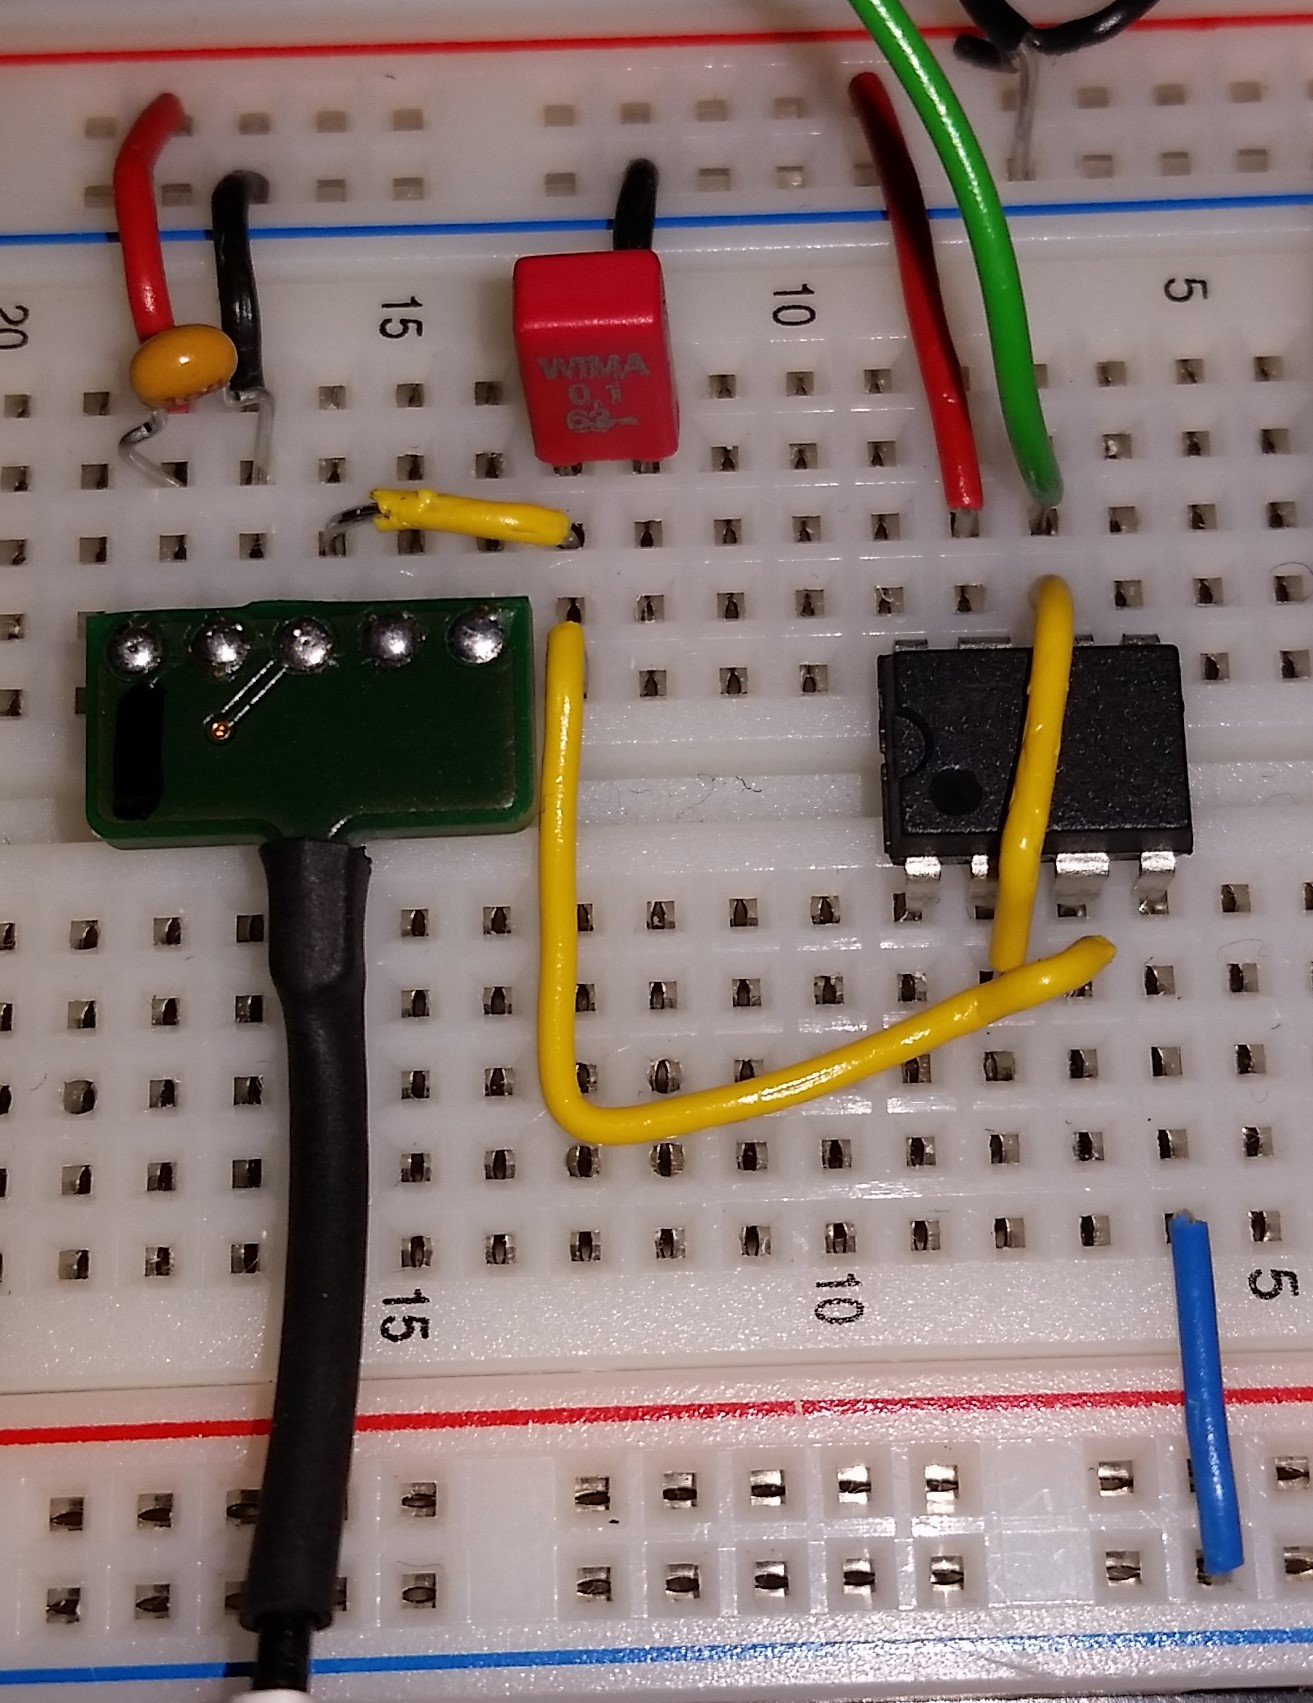
\includegraphics[scale=0.15]{figures/cProblemloesning/PF2.jpg}
	\caption{På billedet ses opsætningen på breadboardet. De røde ledninger symboliserer den positive spænding fra den $5.5$V spændingsforsyning. De sorte ledninger leder til ground, og den blå ledning symboliserer den negative spænding fra spændingsforsyning. De gule ledning fungerer som ledere for signalet igennem systemet (den gule ledning fra accelerometret kan skiftes imellem pin $3$, $4$ og $5$ alt efter hvilken akse, der skal måles på). Den grønne ledning symboliserer outputtet fra kredsløbet, som sendes til NI USB-6009.}
	\label{pforsoeg1}
\end{figure}

\subsection{Fremgangsmåde}
\subsubsection{Forsøgets udførelse}
Hele pilotforsøgets opsætning ses på \figref{pforsoeg2}. \\
For at måle $0g$ påvirkning på accelerometerets x-akse, lægges det fladt ned på et plant bord, som er tjekket med et vaterpas. Målingen gøres over tre omgange i $30$ sekunder. Herefter holdes accelerometeret fast på en vinkel, hvor ledningerne påsættes med hæftemasse. Accelerometeret sættes så der igen måles på x-aksen, når der sker en rotation til højre og venstre. Vinklen sættes således, at der måles $1g$ påvirkning i positiv retning og negativ retning, hvilket svarer til $\pm90^{\circ}$ fra accelerometerets nulpunkt. \\
Dette giver tre baselines for hver g påvirkning, som opsamles og gemmes i ScopeLogger. %Herudover måles en baseline for g påvirkningen af accelerometeret ved $8^{\circ}$ og $13^{\circ}$. Dette gøres ved at holde accelerometeret i 30 sekunder på $8^{\circ}$ og $13^{\circ}$ henholdsvis til højre og venstre. Herved fås 4 baselines, som optages og gemmes i ScopeLogger. 
Til sidst måles g påvirkningen af accelerometeret under rotation fra $0^{\circ}$ til $\pm$ $90^{\circ}$ for både højre og venstre. Her måles $10$ sekunders baseline inden og efter rotationen, som varer $5$ sekunder og foretages langsomt og kontrolleret. Disse to målinger optages og gemmes ligeså i ScopeLogger. \\
\subsubsection{Behandling af data}
Efter udførelse af forsøget vil alt data blive behandlet i MATLAB R2015a, hvor der beregnes en gennemsnitsværdi for henholdsvis de tre baselines målt ved $0g$ påvirkning samt $1g$ påvirkning i positiv retning og negativ retning. Der foretages desuden en Fast Fourier Transformation (FFT) på de ni målinger (tre målinger ved hver g påvirkning). FFT foretages for at få en grafisk repræsentation af det målte signal i frekvensdomænet. Baseline optages for at se hvilken påvirkning omgivelserne har på signalet, da der ikke er nogen bevægelse på disse.

\begin{figure}[H]
	\centering
	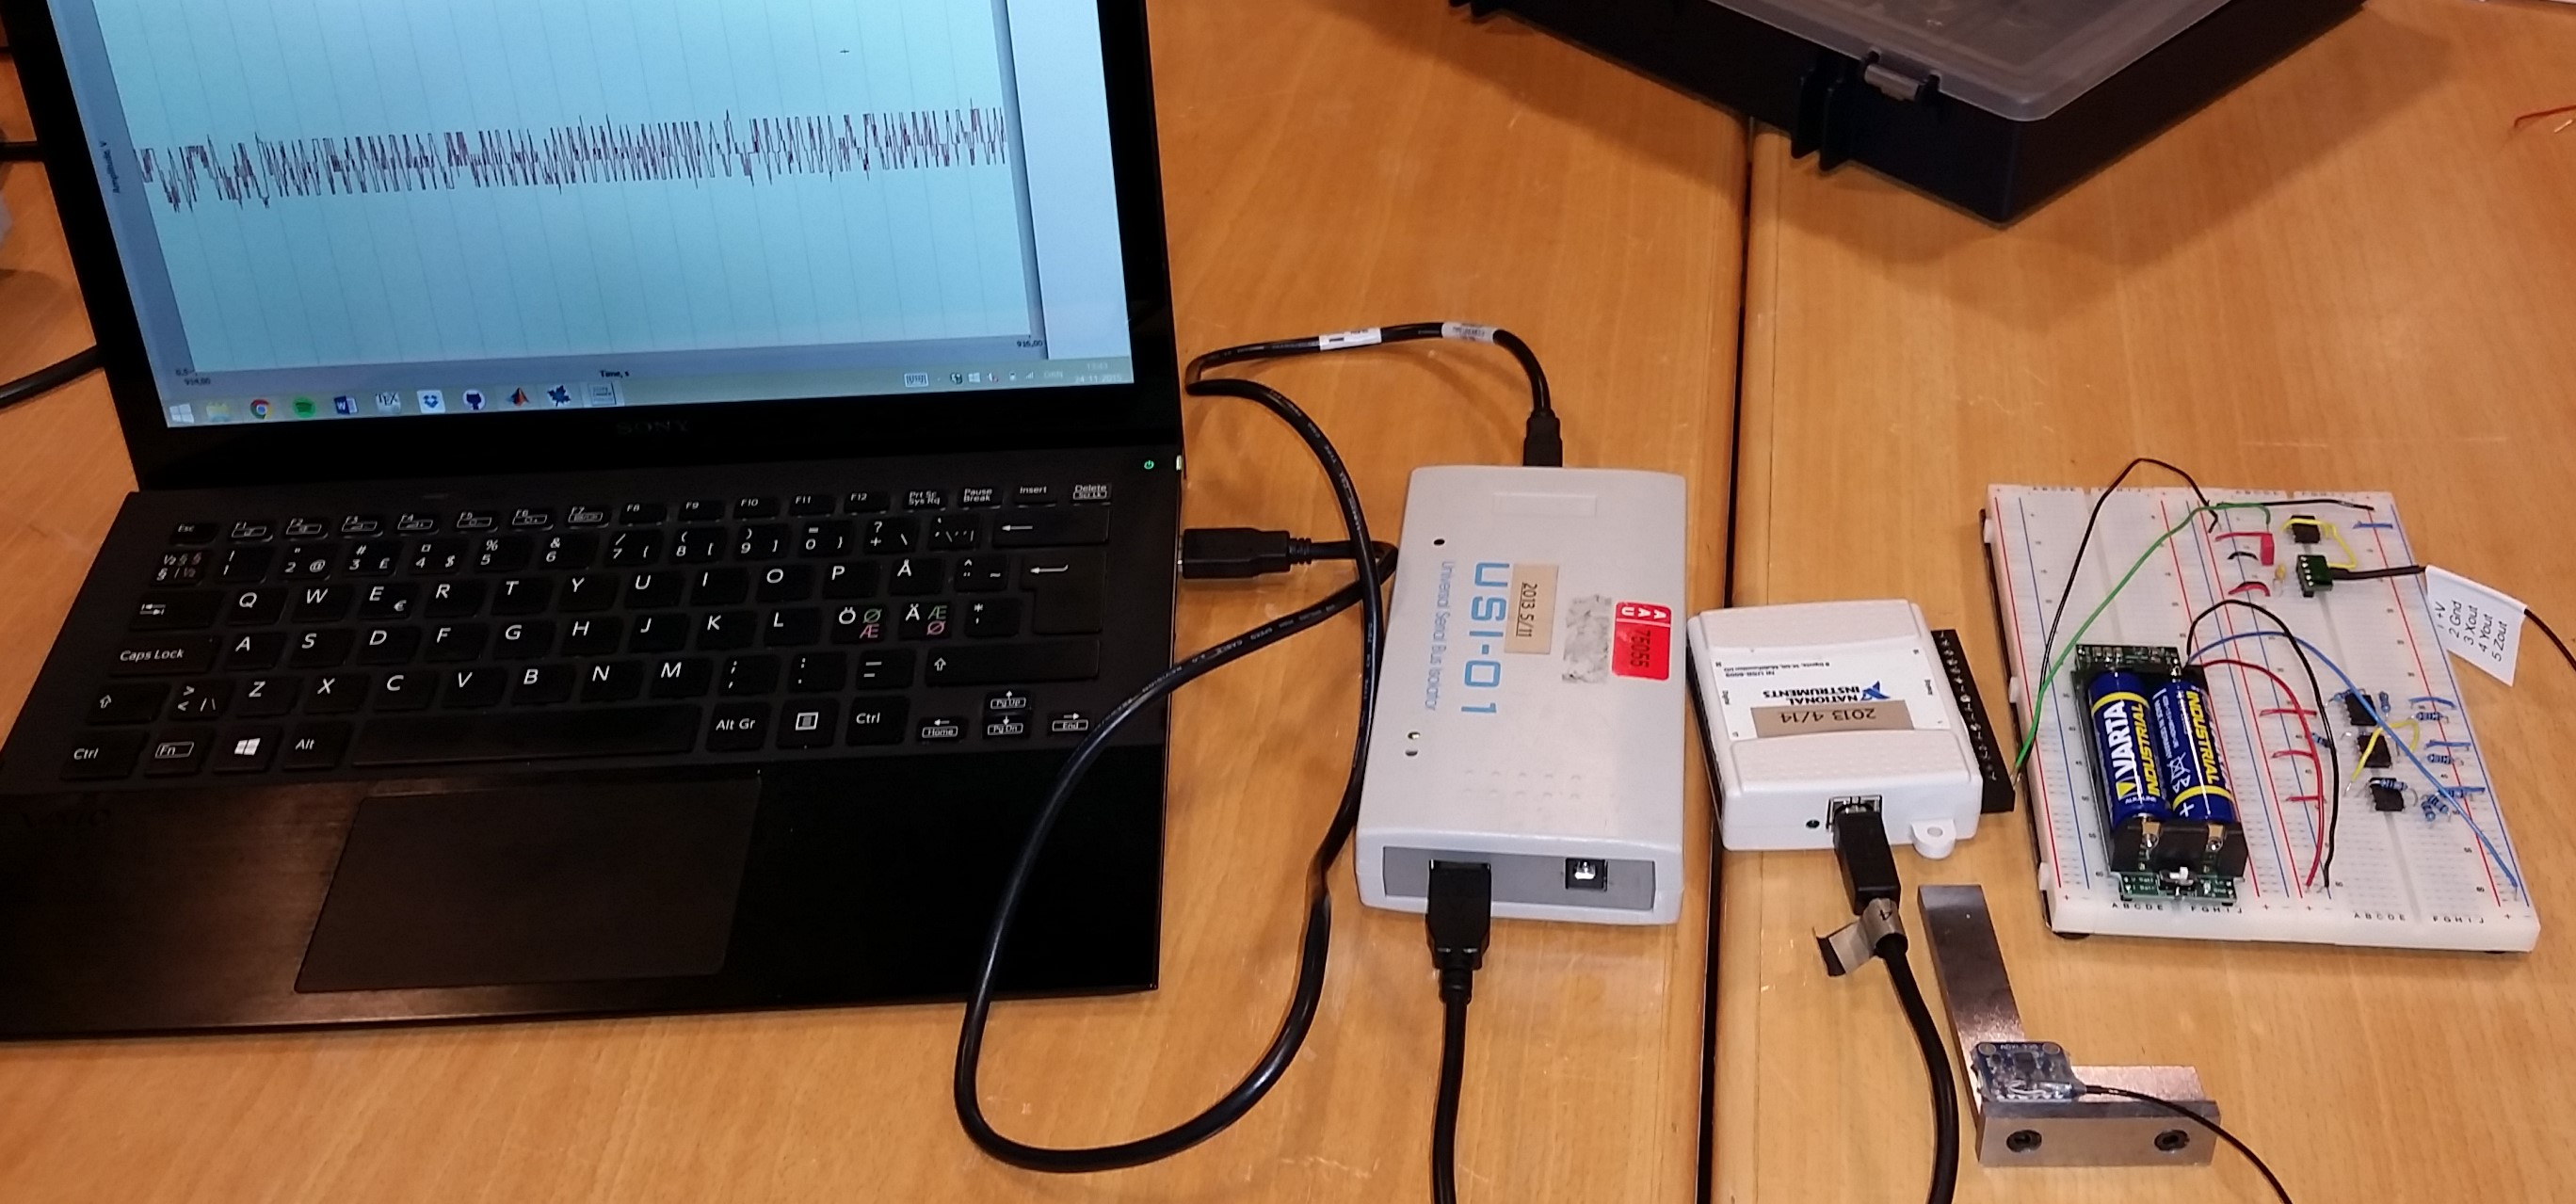
\includegraphics[scale=0.14]{figures/cProblemloesning/Pilotforsoeg1_2.jpg}
	\caption{På billedet ses (fra venstre til højre) den 5V spændingsforsyning, som leder strømmen til og fra ground fra breadboardet. Fra breadboardet sendes outputtet videre til ADC'en(NI USB-6009). Herefter ledes signalet igennem USB-isolatoren(USI-01) og til sidst ind i computeren, hvor det optages i ScopeLogger. Over breadboardet i midten på billedet ses vaterpasset. Forrest i midten på billedet ses accelerometret fastgjort på vinklen.}
	\label{pforsoeg2}
\end{figure}

\subsection{Resultater}\label{Sec_Pilot_Data}
I dette afsnit vil der grafisk blive vist, hvordan accelerometerets output ændrer sig ift. g påvirkning. På \figref{Fig:Pilot_Tid} ses accelerometerets output i tidsdomænet. Der udføres herefter en FFT på de tre målinger for hver baseline, hvilket giver ni grafiske skiltninger af, hvorledes accelerometerets egne frekvenser adskiller sig fra støjfrekvenser.

\begin{figure}[H]
	\centering
	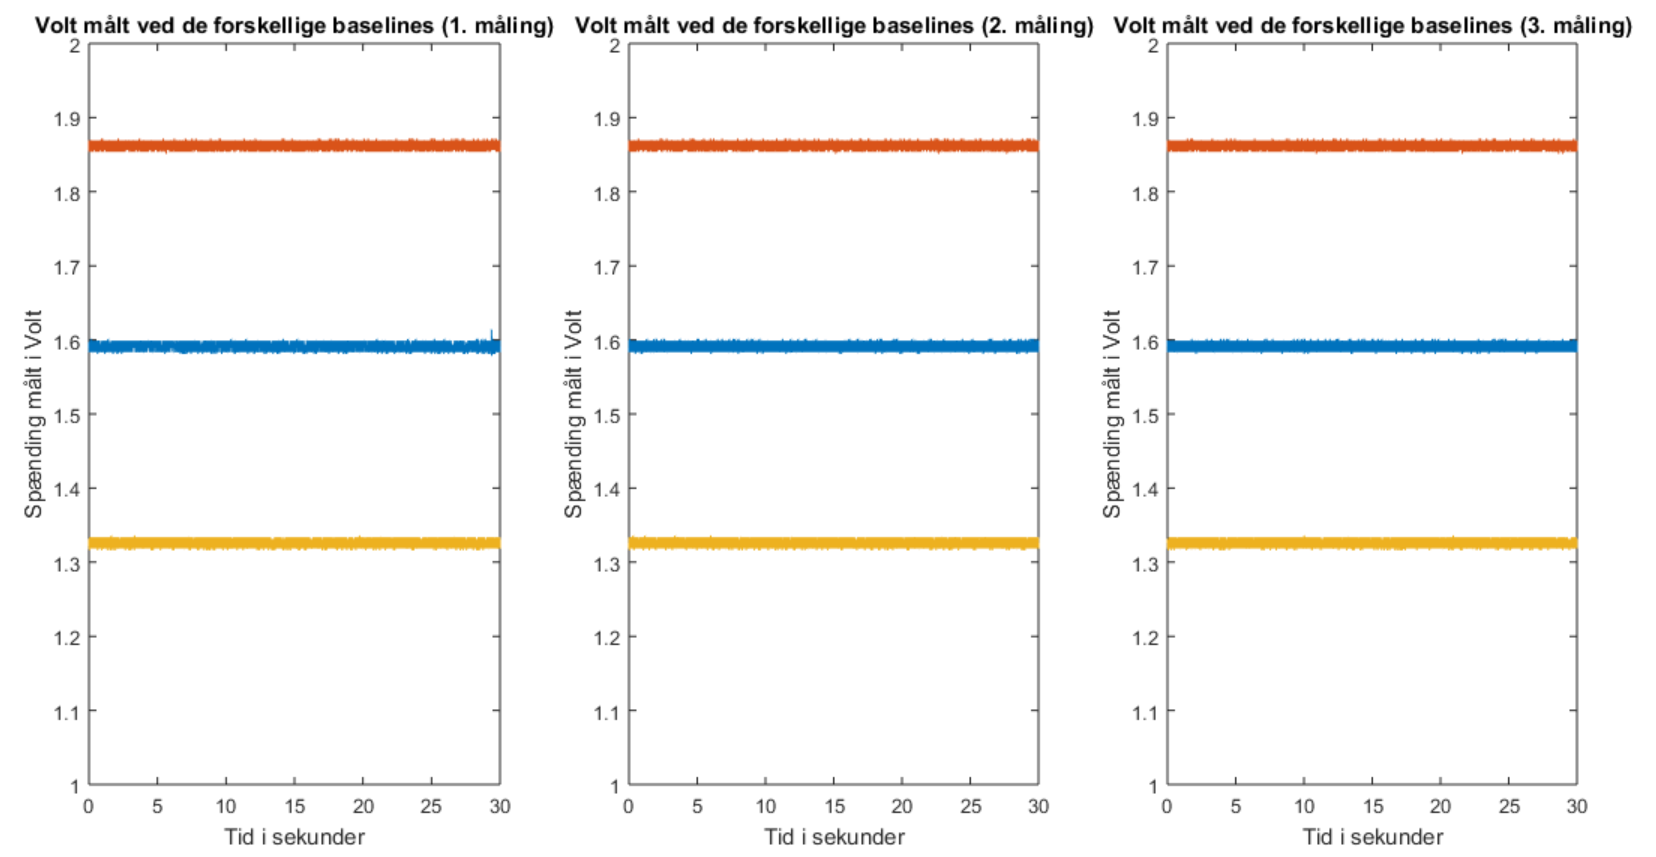
\includegraphics[scale=0.45]{figures/cProblemloesning/Pilotforsoeg_Tid.png}
	\caption{På graferne ses henholdsvis første, anden og tredje måling for hver g påvirkning af accelerometret. Den røde graf repræsenterer outputtet målt ved $1g$ påvirkning i positiv retning. Den blå graf repræsenterer outputtet målt ved $0g$ påvirkning. Den gule graf repræsenterer outputtet målt ved $1g$ påvirkning i negativ retning.}
	\label{Fig:Pilot_Tid}
\end{figure}

Offsettet for accelerometerets x-akse udregnes ved at tage den målte gennemsnitsværdi ved $0$g for alle tre målinger og yderligere tage gennemsnittet af disse. De tre målinger ses som de blå grafer på \figref{Fig:Pilot_Tid}. Udregningen ses på \ref{Mean_tid_0g}:
\begin{equation}\label{Mean_tid_0g}
\text{Offset} = \frac{1.6326 + 1.6323 + 1.6325}{3} = 1.6325
\end{equation}
\noindent Offsettet burde ifølge databladet for accelerometret være halvdelen af spændingsforsyningen, som i dette tilfælde leder en spænding på $3.3V$. \cite{Devices2009} Derfor burde offsettet være $1.65V$. Afvigelsen kan derved udregnes:
\begin{equation}
\text{Afvigelse for offset} = \dfrac{1.6325 - 1.65}{1.65} \cdot 100 = -1.0614\% \approx 1.06\%
\end{equation}

\noindent Herefter kan sensitiviteten for accelerometeret udregnes. Dette gøres ved først at udregne en gennemsnitsværdi for $1g$ påvirkning i henholdsvis positiv og negativ retning. Værdierne for $1$g påvirkning i positiv retning er angivet som de røde grafer på \figref{Fig:Pilot_Tid}, imens de i negativ retning er angivet som de gule grafer. Efter udregningen af gennemsnittet trækkes den udregnede offset værdi fra.
\begin{align}
	\text{Gennemsnit 1g positiv retning} = \frac{1.9640 + 1.9636 + 1.9639}{3} = 1.9638 \\
	\text{Gennemsnit 1g negativ retning} = \frac{1.3091 + 1.3093 + 1.3093}{3} = 1.3092 \\
	\text{Sensitivitet positiv retning} = 1.9638 - 1.6325 = 0.3313 \\
	\text{Sensitivitet negativ retning} = 1.3092 - 1.6325 = -0.3233 \\
	\text{Volt pr grad positiv retning} = \dfrac{0.3313}{90} = 0.0037\text{V}
	\text{Volt pr grad negativ retning} = \dfrac{-0.3233}{90} = 0.0036\text{V}
\end{align}
\noindent Da der findes en lineær sammenhæng imellem g påvirkning og outputtet burde sensitiviteten for accelerometret med en spændingsforsyning på $3.3V$ være $330mV/g$. Der kan derved udregnes afvigelse for både negativ og positiv retning:
\begin{align}
	\text{Afvigelse for sensitivitet i positiv retning} = \dfrac{0.3313 - 0.330}{0.330} \cdot = 0.3939\% \approx 0.39\% \\
	\text{Afvigelse for sensitivitet i negativ retning} = \dfrac{0.3233 - 0.330}{0.330} \cdot = -2.0303\% \approx 2.03\%
\end{align}

På \figref{Fig:Pilot_FFT0}, \figref{Fig:Pilot_FFTN} samt \figref{Fig:Pilot_FFTP} ses en FFT af det målte data for statisk acceleration.
\begin{figure}[H]
	\centering
	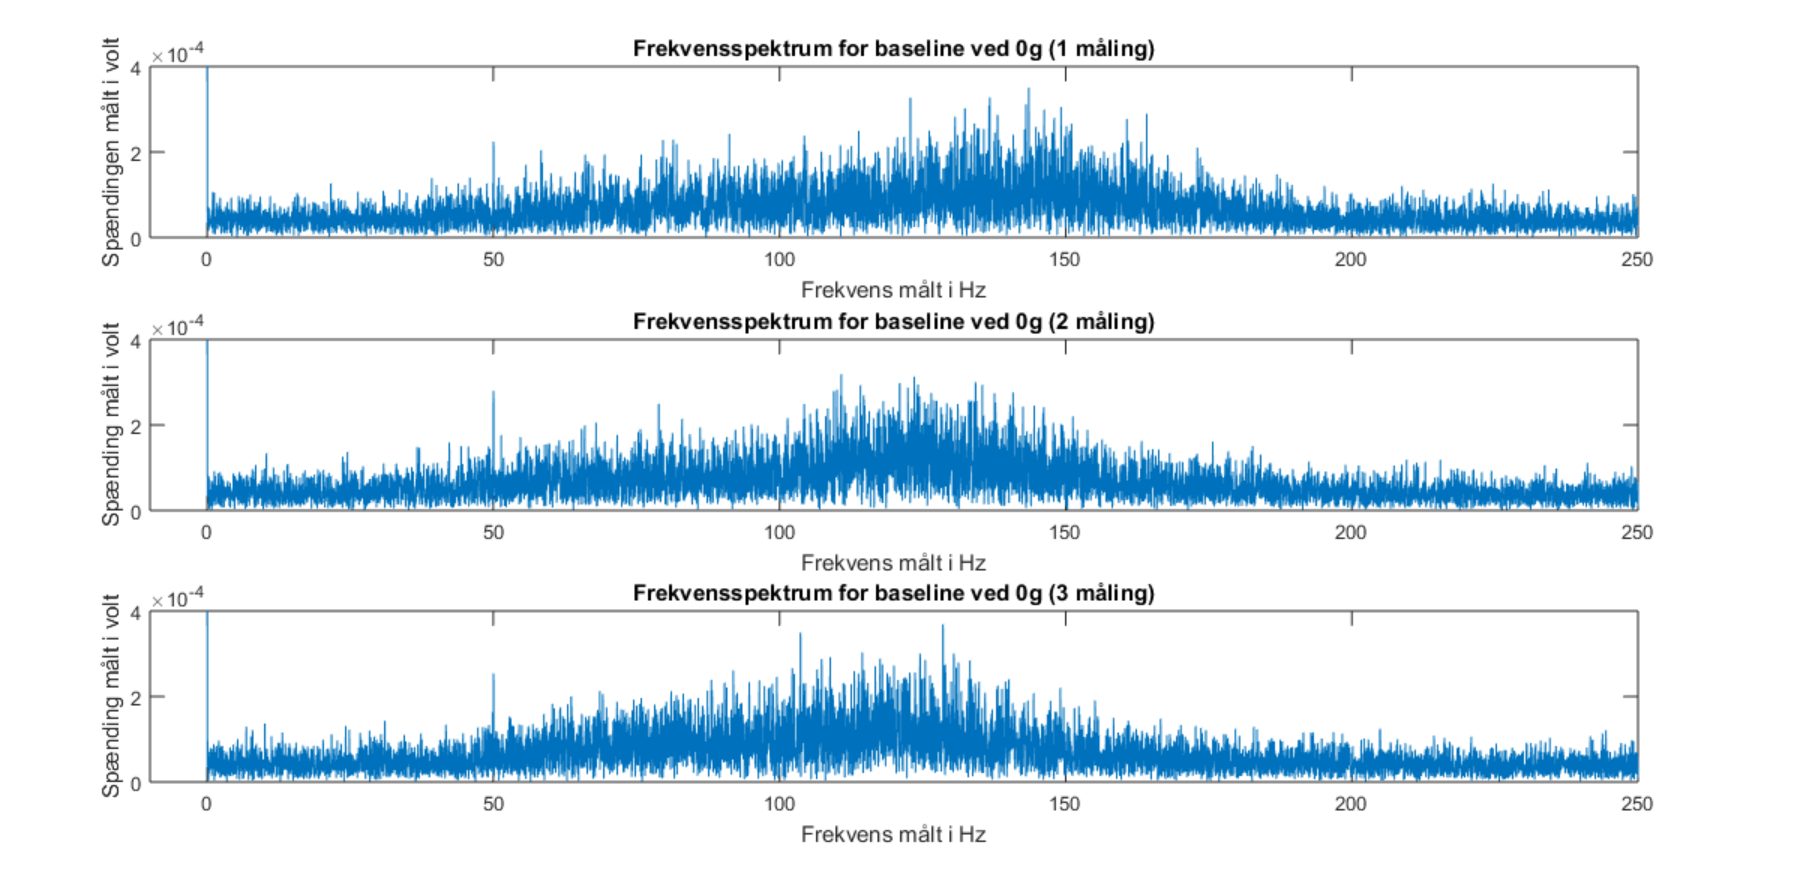
\includegraphics[scale=0.5]{figures/cProblemloesning/Pilotforsoeg_Frekvens0.png}
	\caption{På de tre grafer ses en FFT af første, anden og tredje måling ved $0g$ påvirkning af accelerometret. Peaken ved $0Hz$ går op til ca. $1.63V$ men dette ses ikke på grafen, da resten af værdierne derved vil være meget svære at se.}
	\label{Fig:Pilot_FFT0}
\end{figure}
\begin{figure}[H]
	\centering
	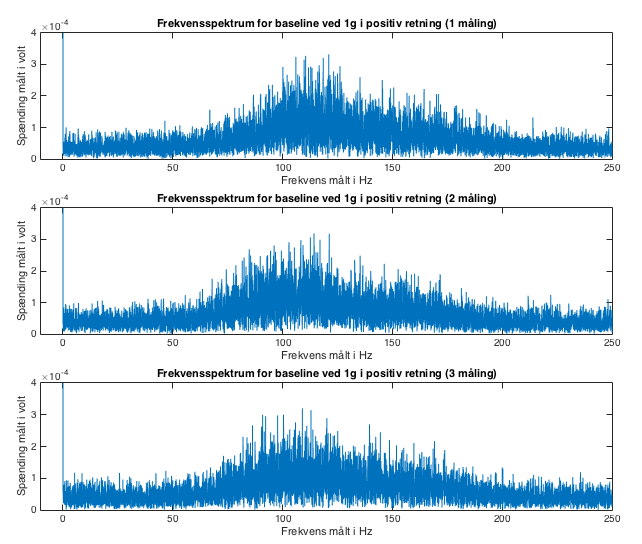
\includegraphics[scale=0.5]{figures/cProblemloesning/Pilotforsoeg_FrekvensP.png}
	\caption{På de tre grafer ses en FFT af første, anden og tredje måling ved $1g$ påvirkning af accelerometret i positiv retning. Peaken ved $0Hz$ går op til ca. $1.96V$, men dette ses ikke på grafen, da resten af værdierne derved vil være meget svære at se.}
	\label{Fig:Pilot_FFTP}
\end{figure}
\begin{figure}[H]
	\centering
	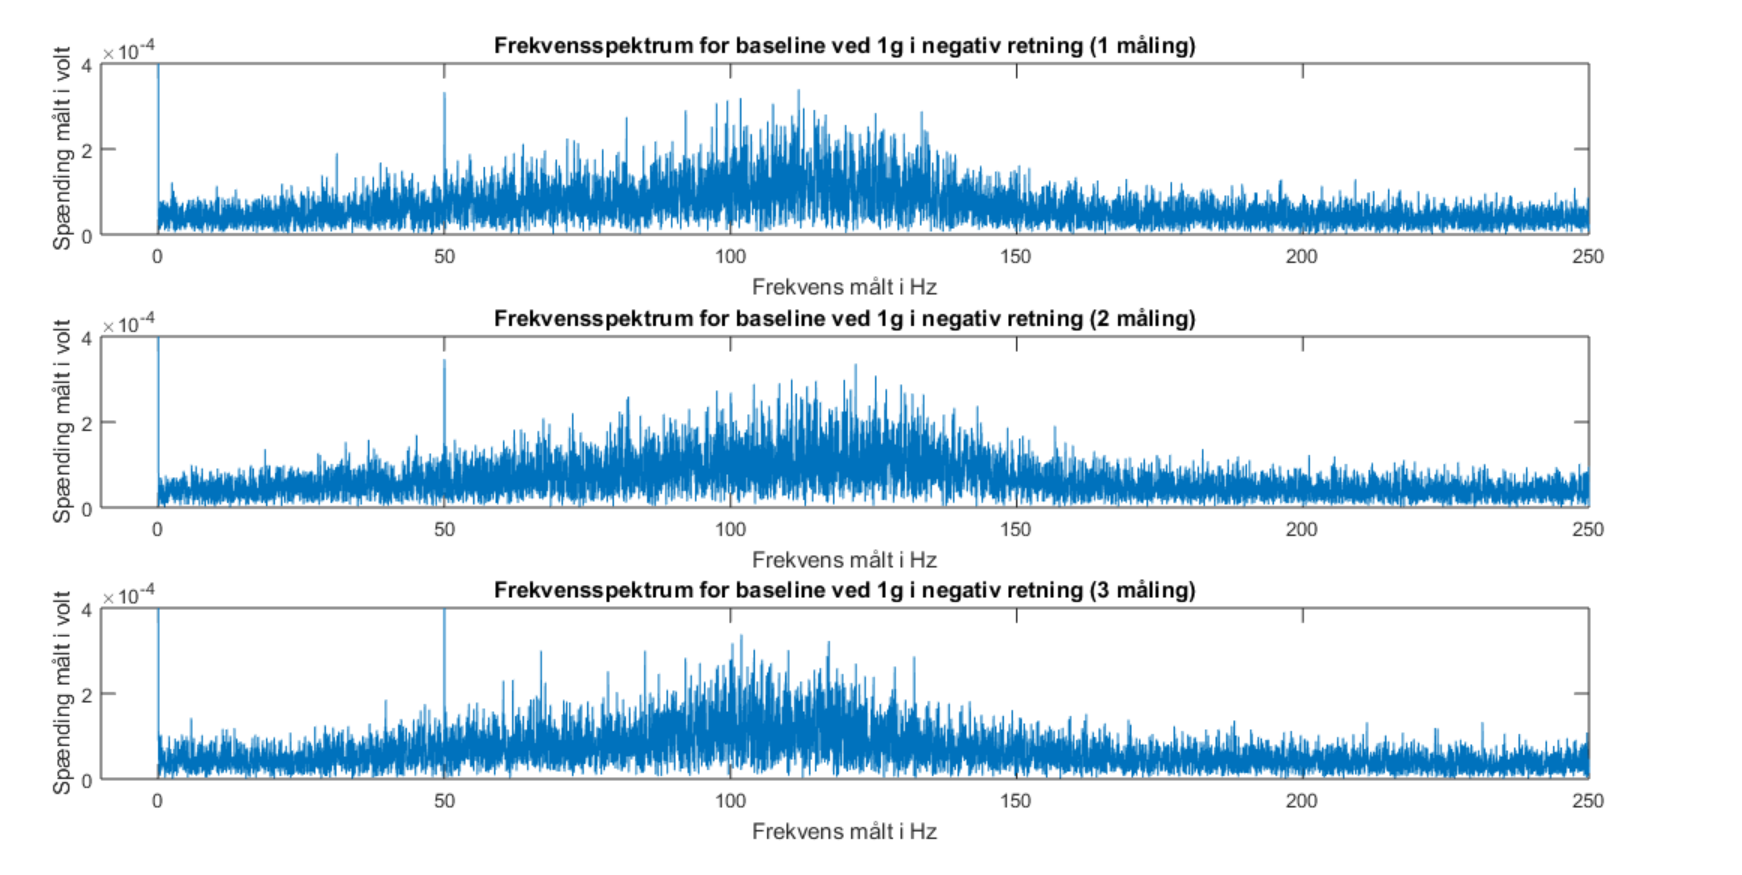
\includegraphics[scale=0.5]{figures/cProblemloesning/Pilotforsoeg_FrekvensN.png}
	\caption{På de tre grafer ses en FFT af første, anden og tredje måling ved -$1g$ påvirkning af accelerometret i negativ retning. Peaken ved $0Hz$ går op til knap $1.30V$, men dette ses ikke på grafen, da resten af værdierne derved vil være meget svære at se.}
	\label{Fig:Pilot_FFTN}
\end{figure}

\noindent Sammenlignes peakværdierne ved $0Hz$ på de tre ovenstående figurer med peakværdierne i resten af signalet fremgår det, at signal to noise ratioen er lav, hvilket betyder, at der ikke er meget støj ift. ønsket signal. Der ses altså, at accelerometerets frekvensområde ligger i de lave frekvenser. Der ses ved en statisk acceleration at, signalet stort set kun er til stede ved $0Hz$. Alt over $0Hz$ betragtes derfor som støj. 

\begin{figure}[H]
	\centering
	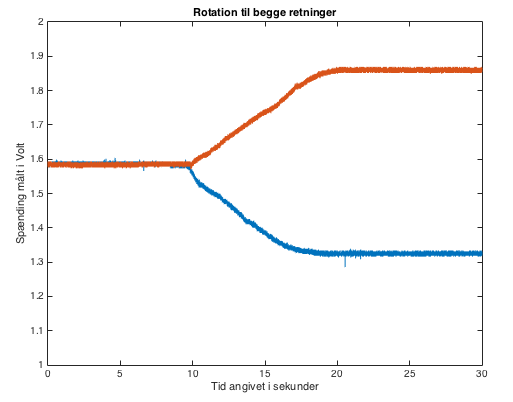
\includegraphics[scale=0.45]{figures/cProblemloesning/Pilotforsoeg_Rotation.png}
	\caption{På graferne ses accelerometerets output ved rotation fra $0g$ påvirkning til $1g$ påvirkning. Den orange graf repræsenterer rotation i positiv retning, hvorimod den blå graf repræsenterer rotation i negativ retning.}
	\label{Fig:Pilot_Rottid}
\end{figure}
\begin{figure}[H]
	\centering
	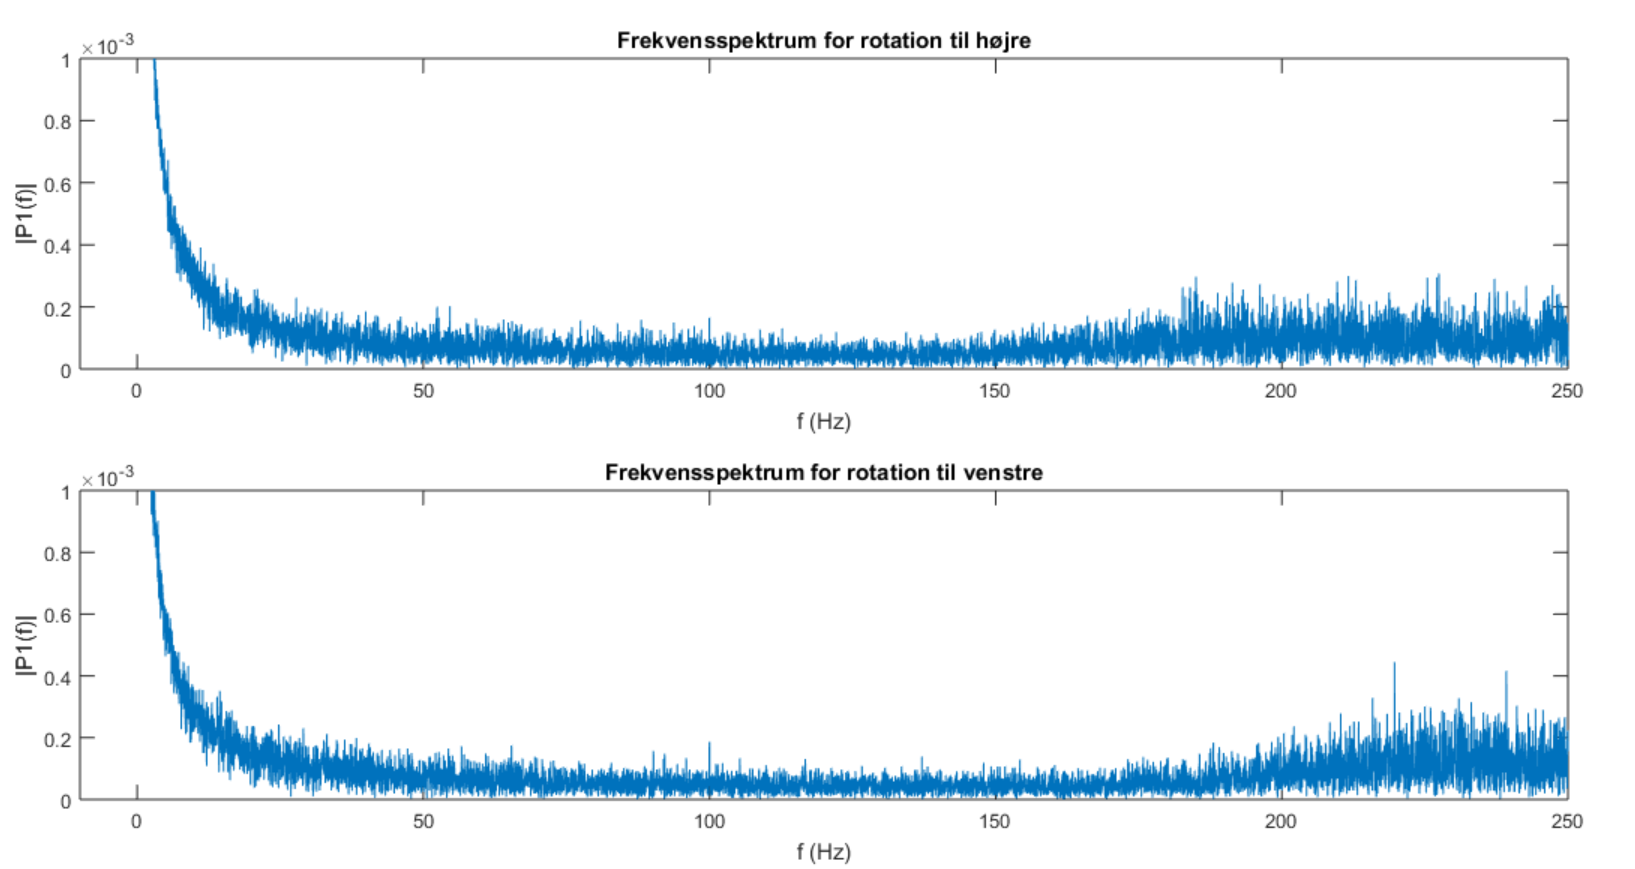
\includegraphics[scale=0.5]{figures/cProblemloesning/Pilotforsoeg_RotationFrekvens.png}
	\caption{På graferne ses en FFT af målinger for rotation i henholdsvis positiv og negativ retning.}
	\label{Fig:Pilot_Rotfrek}
\end{figure}
På \figref{Fig:Pilot_Rottid} ses der en lineær sammenhæng imellem g-påvirkning af accelerometret og outputtet. Der ses, at de tre baselines ved $0g$ påvirkning samt $1$g påvirkning i henholdsvis positiv og negativ retning, som måles i de første og sidste $10$ sekunder af målingen, stemmer overens med de målte baselines uden rotation. \\
På \figref{Fig:Pilot_Rotfrek} ses en FFT af målingerne af rotationerne. Ud fra dette kan der ses, at der er kommet større udsving i de lavere frekvenser fra $0-$ til ca. $25Hz$ sammenlignet med de statiske baseline målinger. Signalet regnes altså for at være i frekvensspektrummet $0-25Hz$. Alt uden for dette spektrum regnes derfor som støj.

\subsection{Diskussion og konklusion}
Der kan argumenteres for og imod at accelerometret er blevet udsat for $0g$ påvirkning, da det kan være svært at vurdere hvorvidt bordet er plant. Bordets hældning blev målt med et vaterpas, men der er mulighed for, at vaterpasset kan være upræcist. Accelerometret har desuden ujævnheder på overfladen i form af ledninger, hvilket kan betyde, at det muligvis ikke har lagt plant på bordet. \\
Der kan også være faktorer som har betydning for $1g$ påvirkningen, da vinklen nødvendigvis ikke er helt vinkelret. Ujævnheder på accelerometret samt vores holdemåde på det kan også have påvirket målingen. \\
Accelerometerets output afhænger også af rumtemperaturen, da denne påvirker aksernes offset samt sensitiviteten. Ved dette forsøg var temperaturen før, under og efter forsøget {\color{red}X, X og X}, hvilket vil gå ind og påvirke målingerne. \\
Alle disse faktorer som er udregnet for pilotforsøget kan have indflydelse på de afvigelser der fås ift. databladet for accelerometeret. Det er altså igennem forsøget lykkedes at udregne afvigelserne for offset samt sensitiviteten, som står i accelerometrets datablad.  \\

I outputsignalet fra accelerometret ved den statiske acceleration udgør alt over $0Hz$ støj, hvorimod det vurderes, at alt over $25$Hz for rotationsmålingerne er støj. Maksimum og minimum outputsignalet fra accelerometret vil for langsom rotation eller svajning henholdsvis være $1.9638$V og $1.3092$V, hvilket bliver til $0.3313V$ og -$0.3233V$ efter offsettet er blevet justeret, der udregnes til $0.0037$V og -$0.0036$V pr grad. \\